
%% ==================================================================================================
%%
\documentclass[12pt]{book}
\usepackage{amsfonts}
\usepackage{amsmath}
\usepackage{amssymb}
\usepackage{graphicx}
\usepackage{hyperref}
\usepackage{float}
\usepackage{verbatim}
\usepackage{xlop} %% for multiplication https://tex.stackexchange.com/questions/11702/how-to-present-a-vertical-multiplication-addition
\usepackage{listings} %% to format generic computer code
\usepackage{lmodern} % for bold teletype font
\usepackage{minted} % colour Java code

\usepackage{tasks}
%\NewTasks[style=enumerate,counter-format=tsk[A].,label-width=3ex]{choice}[\item](4)

%% =======   set page margins    =======
\setlength{\textheight}{10in}
\setlength{\textwidth}{7.4in}
\setlength{\topmargin}{-0.75in}
\setlength{\oddsidemargin}{-0.5in}
\setlength{\evensidemargin}{-0.5in}
\setlength{\parskip}{0.15in}
\setlength{\parindent}{0in}

%%  for European long division
% https://tex.stackexchange.com/questions/432435/how-to-set-up-european-french-style-long-division-in-tex
\newcommand\frdiv[5]{%
    \[
    \renewcommand\arraystretch{1.5}
    \begin{array}{l| l}
    #1 & #2 \\
    \cline{2-2}
    #3 & #4 \\
    \cline{1-1}
    #5 & \\
    \end{array}
    \]
}

%%  for European long division


%% ==================================================================================================

\begin{document}

%\title{ITI1100 Digital Systems I}
%\author{Kien Do 300163370}
%\date{Assignment \#1}
\newcommand{\reporttitle}{Devoir 1}
\newcommand{\reportauthorOne}{Kien Do}
\newcommand{\cidOne}{300163370}
\input{titlePage/titlepage.txt}



%% ==================================================================================================

%%%%%%%%%%%% PROBLEMS START HERE

\begin{enumerate}
    \item \textbf{Réponse}
\begin{minted}[breaklines,frame=single]{java}
<assign> -> <id> = <expr>
<id> -> A | B | C
<expr> -> <expr> * <term>
        | <term>
<term> -> <factor> + <term>
        | <factor>
<factor> -> ( <expr> )
        | <id>
\end{minted}
    \item \textbf{Réponse}\\
    
    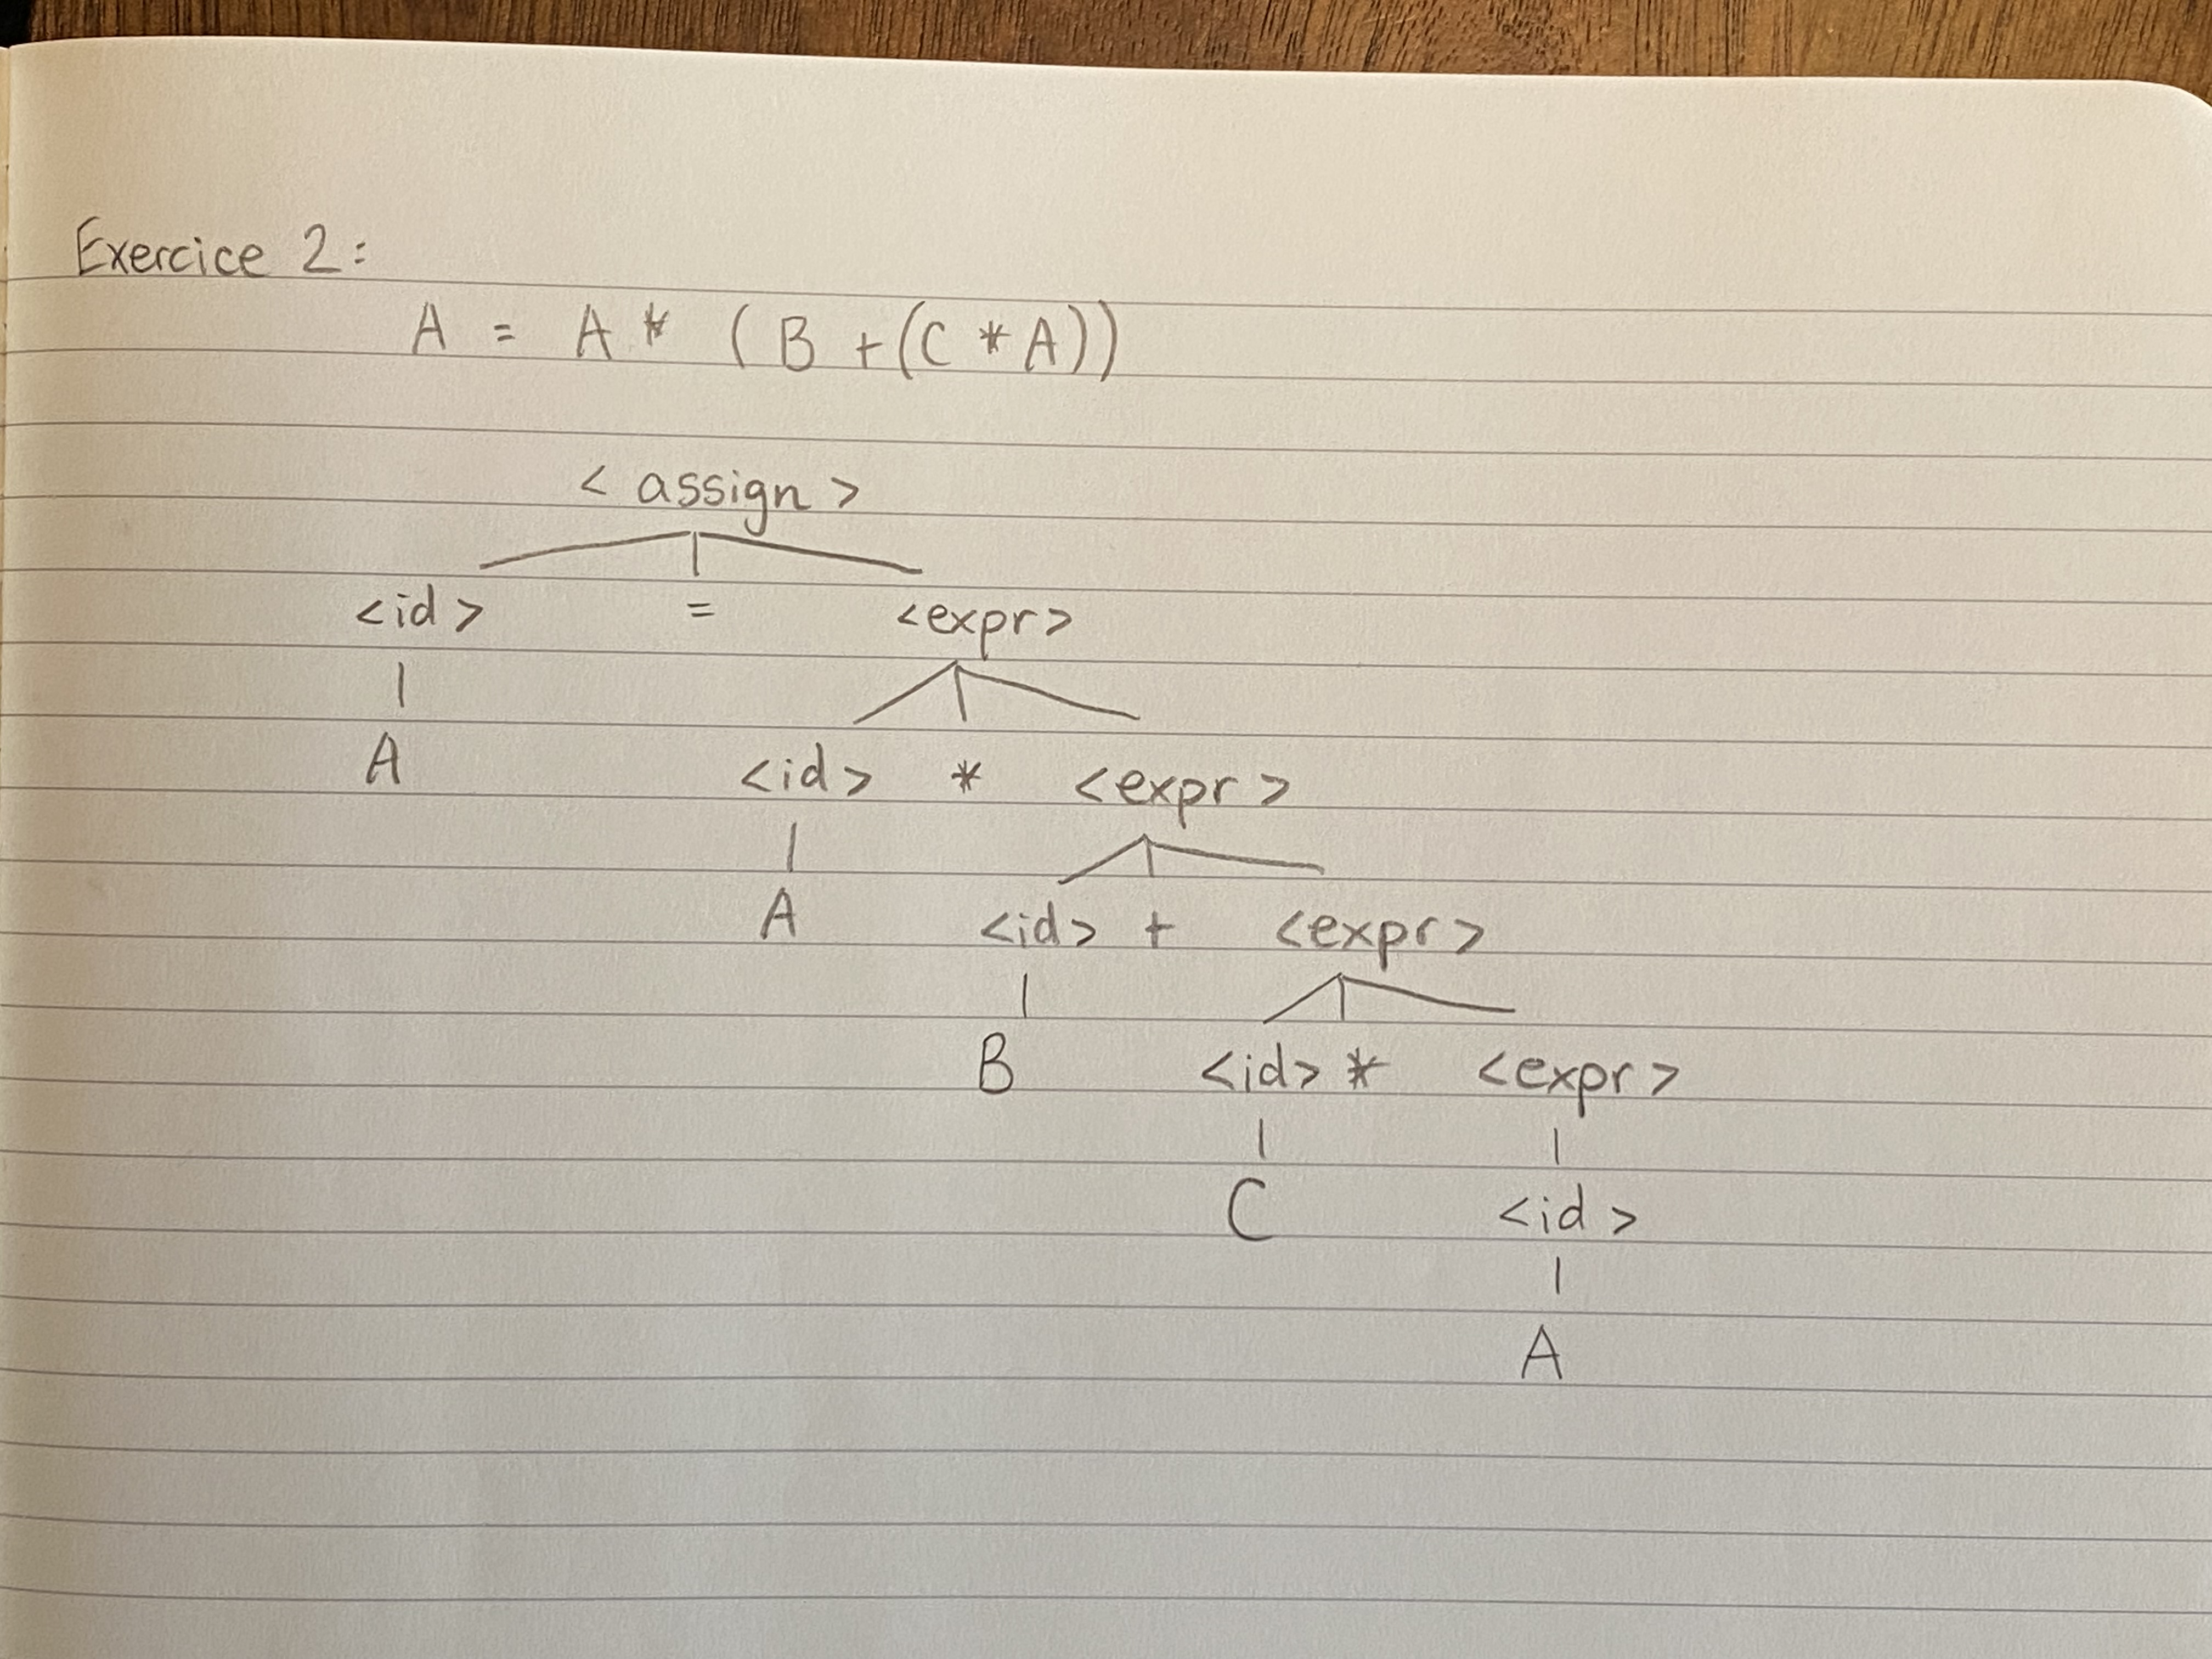
\includegraphics[scale=0.12]{ex2.png}
    
    \newpage
    
    \item \textbf{Réponse}\\
    
    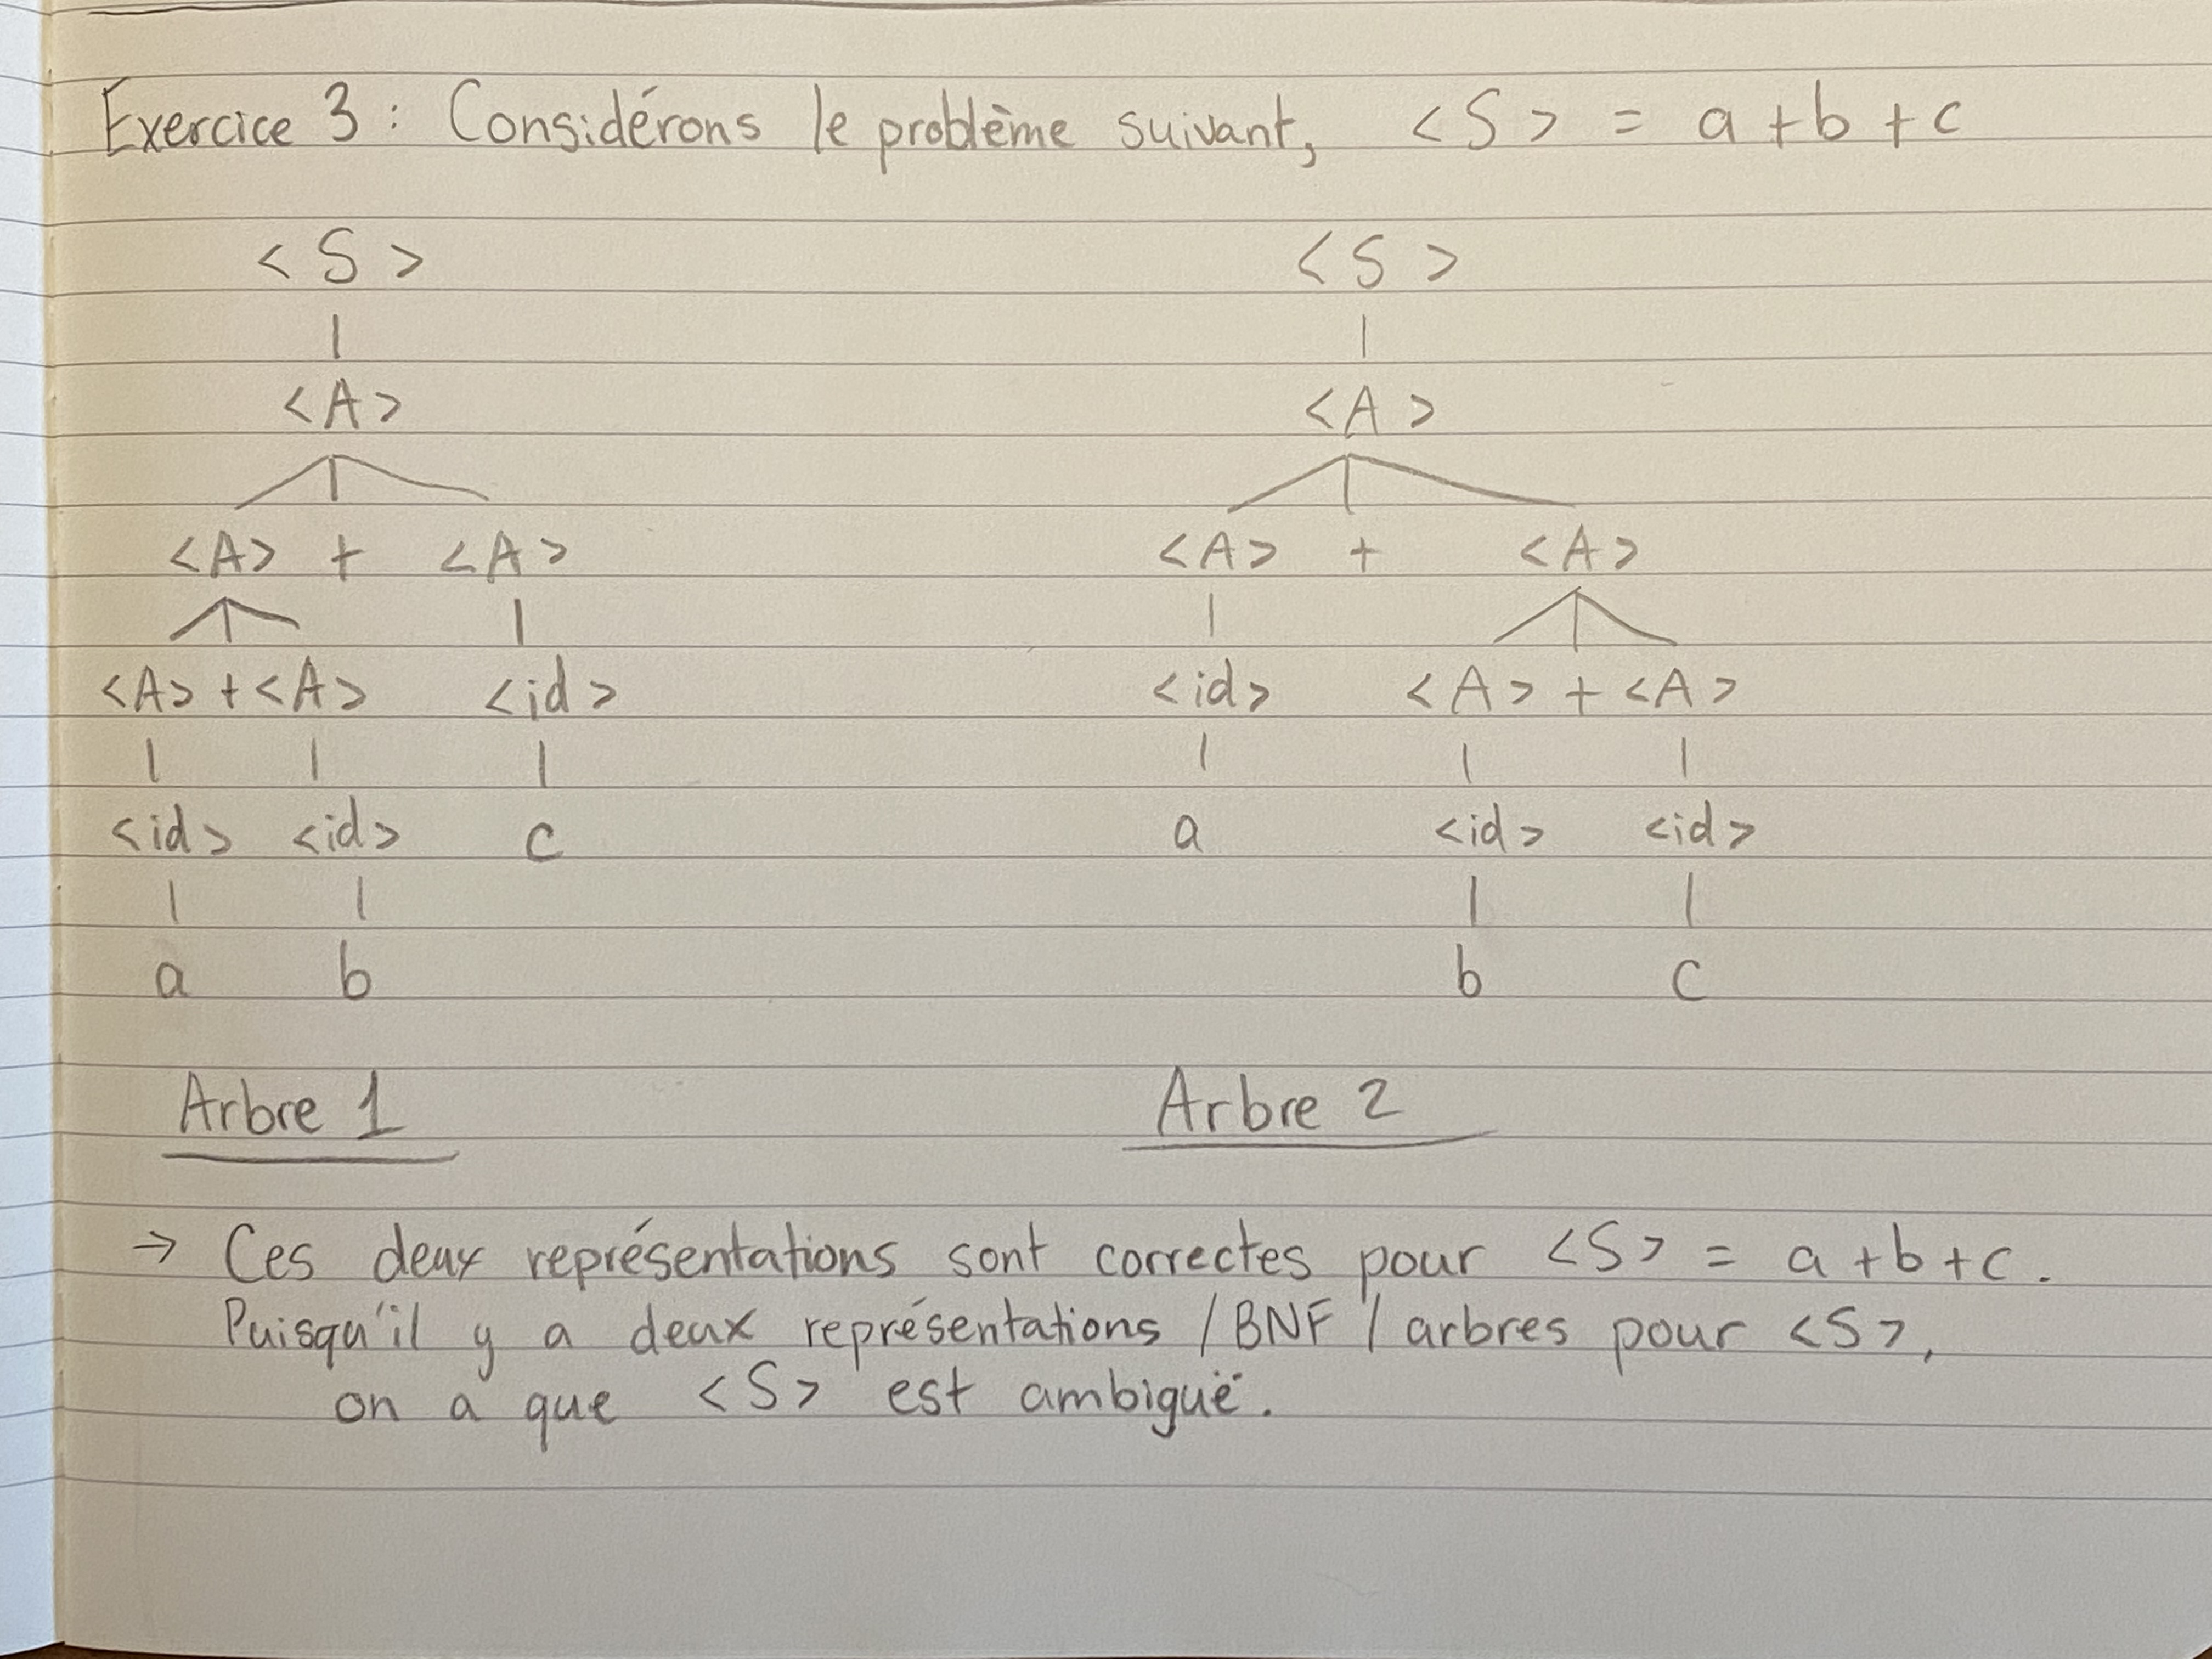
\includegraphics[scale=0.12]{ex3.png}
    
    \item \textbf{Réponse}
\begin{minted}[breaklines,frame=single]{java}
<assign> -> <id> = <expr>
<id> -> A | B | C
<expr> -> <expr> {( + | * ) <expr>}
        | ( <expr> )
        | <id>
\end{minted}

    \item \textbf{Réponse}
    \begin{enumerate}
        \item 
\begin{minted}[breaklines,frame=single]{java}
M_r (repeat L until B)
    if M_b (B, s) = undefined | M_sl (L, s) = error
        then error
        else if M_b(B, s) = true
            then M_sl (L, s)
        else
            M_r (repeat L until B, M_sl (L, s))
\end{minted}
\newpage
%         \item
% \begin{minted}[breaklines,frame=single]{java}
% M_b (B, s)
%     if VARMAP(i, s) = undefined for some i in B
%         then error
%     else B', where B' is the result of evaluating B after setting each variable i in B to VARMAP(i, s)
% \end{minted}
    \end{enumerate}
    
    \item \textbf{Réponse}
    \begin{enumerate}
        \item 
        Puisque $$a = 2 * (b - 1) - 1 \qquad \{a > 0\}$$ On a que,
        \begin{align*}
            a &> 0\\
            2 * (b - 1) - 1 &> 0\\
            2b - 2 - 1 &> 0\\
            2b - 3 &> 0\\
            b &> 3/2
        \end{align*}
        \item 
        Puisque $$b = (c+10) / 3  \qquad \{b > 6\}$$ On a que,
        \begin{align*}
            b &> 6\\
            (c+10) / 3 &> 6\\
            c + 10 &> 18\\
            c &> 8
        \end{align*}
    \end{enumerate}
    
    \item \textbf{Réponse}\\
    
        Puisque
        \begin{align*}
            a &= 2b + 1\\
            b &= a - 3 \qquad \{b < 0\}
        \end{align*}
        On peut dire que
        \begin{align*}
            b &< 0\\
            a - 3 &< 0\\
            a &< 3
        \end{align*}
        Et donc,
        \begin{align*}
            a &= 2b + 1 \qquad \{a < 3\}\\
            a &< 3\\
            2b + 1 &< 3\\
            2b &< 2\\
            b &< 1
        \end{align*}


\end{enumerate}






\end{document} 
